\documentclass[a4paper, 10pt, twoside]{article}

\usepackage[top=1in, bottom=1in, left=1in, right=1in]{geometry}
\usepackage[utf8]{inputenc}
\usepackage[spanish, es-ucroman, es-noquoting]{babel}
\usepackage{setspace}
\usepackage{fancyhdr}
\usepackage{lastpage}
\usepackage{amsmath}
\usepackage{amsfonts}
\usepackage{amsthm}
\usepackage{svg}
\usepackage{amsmath}
\usepackage{graphicx}
\usepackage{xcolor}
\usepackage{float}
\usepackage{svg}
\usepackage{enumitem} % Provee macro \setlist
\usepackage{tabularx}
\usepackage{multirow}
\usepackage{hyperref}
\usepackage{multicol}
\usepackage{verbatim}
\usepackage[procnames]{listings}
\usepackage[toc, page]{appendix}
\usepackage{color}
\usepackage{syntax}

\usepackage{subfig}


%%%%%%%%%% Configuración de Fancyhdr - Inicio %%%%%%%%%%
\pagestyle{fancy}
\thispagestyle{fancy}
\lhead{Trabajo Práctico · Teoria de Lenguajes}
\rhead{Rodriguez · Pizzagalli}
\renewcommand{\footrulewidth}{0.4pt}
\cfoot{\thepage /\pageref{LastPage}}

\fancypagestyle{caratula} {
   \fancyhf{}
   \cfoot{\thepage /\pageref{LastPage}}
   \renewcommand{\headrulewidth}{0pt}
   \renewcommand{\footrulewidth}{0pt}
}
%%%%%%%%%% Configuración de Fancyhdr - Fin %%%%%%%%%%


%%%%%%%%%% Miscelánea - Inicio %%%%%%%%%%
% Evita que el documento se estire verticalmente para ocupar el espacio vacío
% en cada página.
\raggedbottom

% Deshabilita sangría en la primer línea de un párrafo.
\setlength{\parindent}{0em}

% Separación entre párrafos.
\setlength{\parskip}{0.5em}

% Separación entre elementos de listas.
\setlist{itemsep=0.5em}

% Asigna la traducción de la palabra 'Appendices'.
\renewcommand{\appendixtocname}{Apéndices}
\renewcommand{\appendixpagename}{Apéndices}
%%%%%%%%%% Miscelánea - Fin %%%%%%%%%%


%%%%%%%%%% Insertar diagrama - Inicio %%%%%%%%%%
\newcommand{\diagramav}[1]{%
  \includegraphics[type=pdf,ext=.pdf,read=.pdf,width=16cm]{diagramas/#1}%
}

\newcommand{\diagramavfig}[2]{%
  \begin{figure}[H]
    \includegraphics[type=pdf,ext=.pdf,read=.pdf,width=16cm]{diagramas/#1}%
    \caption{#2}
    \label{fig:#1}
  \end{figure}
}

\newcommand{\diagramavtrim}[2]{%
  \includegraphics[type=pdf,ext=.pdf,read=.pdf,width=16cm,trim=0 #2 0 0,clip]{diagramas/#1}%
}

\newcommand{\diagramah}[1]{%
  \includegraphics[type=pdf,ext=.pdf,read=.pdf,height=16cm,angle=90]{diagramas/#1}%
}
%%%%%%%%%% Insertar diagrama - Fin %%%%%%%%%%

\newcommand{\subsubfloat}[2]{%
  \begin{tabular}{@{}c@{}}#1\\#2\end{tabular}%
}


\begin{document}


%%%%%%%%%%%%%%%%%%%%%%%%%%%%%%%%%%%%%%%%%%%%%%%%%%%%%%%%%%%%%%%%%%%%%%%%%%%%%%%
%% Carátula                                                                  %%
%%%%%%%%%%%%%%%%%%%%%%%%%%%%%%%%%%%%%%%%%%%%%%%%%%%%%%%%%%%%%%%%%%%%%%%%%%%%%%%


\thispagestyle{caratula}

\begin{center}


\includegraphics[height=2cm]{DC.png}
\hfill

\includegraphics[height=2cm]{UBA.jpg}

\vspace{2cm}

Departamento de Computación,\\
Facultad de Ciencias Exactas y Naturales,\\
Universidad de Buenos Aires

\vspace{4cm}

\begin{Huge}
Trabajo Práctico 1 - Reentrega
\end{Huge}

\vspace{0.5cm}

\begin{Large}
Teoria de Lenguajes
\end{Large}

\vspace{1cm}

Segundo Cuatrimestre de 2015

\vspace{4cm}

\begin{tabular}{|c|c|c|}
\hline
Apellido y Nombre & LU & E-mail\\
\hline
Rodriguez Pedro & 197/12 & pedro3110.jim@gmail.om \\
Matias Pizzagali & 257/12 & matipizza@gmail.com \\
\hline
\end{tabular}

\end{center}

\newpage

\tableofcontents

\section{Correcciones realizadas}
Para la reentrega del TP, realizamos las siguientes modificaciones respecto de la primera entrega:
\begin{itemize}
  \item Rehicimos el código, utilizando clases, aplicando `` buenas prácticas '' de programación
  \item Mejoramos la explicación sobre cómo realizamos el TP; agregamos al informe la TDS que generamos para resolver el problema propuesto
  \item Añadimos casos de test exitosos y fallidos
\end{itemize}

\newpage


\section{Introducción}
El objetivo de este trabajo práctico es desarrollar un compositor de fórmulas matemáticas. El mismo tomará como entrada la descripción de una fórmula en una versión muy simplificada del lenguaje utilizado por LATEX y producirá como salida un archivo SVG (Scalable Vector Graphics).

\section{Desarrollo}
Para poder realizar el TP, utilizamos la librería PLY para Python, la cual implementa Lex y Yacc enteramente en Python. Este analizador léxico y sintáctico nos permitirá aceptar o rechazar cadenas de entrada de acuerdo a la gramática que definamos.

Una de las cosas que tuvimos que hacer para poder utilizar esta herramienta fue definir para este problema en particular los siguientes tokens, con sus respectivas expresiones regulares:
\begin{itemize}
  \item ID : para cualquier caracter distinto a \_, \detokenize{^}, (, ), \{ y \}
  \item SUBINDEX : para la ER `` / ''
  \item SUPERINDEX : para la ER `` \detokenize{^} ''
  \item DIVIDE : para la ER `` /''
  \item LPAREN : para la ER `` ( ''
  \item RPAREN : para la ER `` ) ''
  \item LBRACKET : para la ER `` \{ ''
  \item RBRACKET : para la ER `` \} ''
\end{itemize}

\subsection{Desambiguación de la gramática}

\begin{table}[H]
\begin{tabular} {c c c c c c c}

E & $\rightarrow$ & E & E                 &   & & \\
  & $|$           & E & \detokenize{/}    & E & & \\
  & $|$           & E & \detokenize{^}    & E & & \\
  & $|$           & E & \_                & E & & \\
  & $|$           & E & \detokenize{^}    & E & \_  & E \\
  & $|$           & E & \_                & E & \detokenize{^} & E \\
  & $|$           & \detokenize{(}        & E & \detokenize{)} & & \\
  & $|$           & \{                    & E & \} & & \\
  & $|$           & $l$ & & & & \\
\end{tabular}
\quad \quad \quad \quad \quad \quad \quad \quad \quad \quad
\begin{tabular} {c c c c c c c}

S & $\rightarrow$ & E &                   &   & & \\
E & $\rightarrow$ & E & \detokenize{/}    & A & & \\
  & $|$           & A &                   &   & & \\
A & $\rightarrow$ & A &                   & B & & \\
  & $|$           & B &                   &   & & \\
B & $\rightarrow$ & C &                   &   & & \\
  & $|$           & C & \detokenize{^}    & C & & \\
  & $|$           & C & \_                & C & & \\
  & $|$           & C & \detokenize{^}    & C & \_  & C \\
  & $|$           & C & \_                & C & \detokenize{^} & C \\
C & $\rightarrow$ & \detokenize{(}        & E & \detokenize{)} & & \\
  & $|$           & \{                    & E & \} & & \\
  & $|$           & $l$                  & & & & \\

\end{tabular}
\end{table}

La gramática propuesta inicialmente fue la de la izquierda. Sin embargo, al utilizar esta gramática para hacer el parsing, se generan conflictos Shift/Reduce. Esto es debido a que la gramática es ambigua (para una misma cadena pueden haber más de un árbol de derivación posibles). Luego, para evitar conflictos Shift/Reduce, generamos la otra gramática expuesta, equivalente a la anterior pero con la diferencia de que no es ambigua.

Tuvimos en cuenta que la división es la operación de menor precedencia, seguida de la concatenación, luego los subíndice y superíndice y finalmente los paréntesis y corchetes. También que división y concatenación son asociativas a izquierda y que subíndice y superíndice no son asociativos.

\subsection{TDS y Atributos}
Para cada uno de los símbolos S,A,B,C,E (no terminales) y ID (terminal) definimos los siguientes atributos heredados de tipo float:
\begin{itemize}
  \item $x$ : para guardar el comienzo de cada subexpresión sobre el eje x
  \item $y$ : para guardar el comienzo de cada subexpresión sobre el eje y
  \item $tam$ : para guardar el tamaño (escala) de cada subexpresión
\end{itemize}

Y los siguientes atributos sintetizados, también de tipo float.
\begin{itemize}
  \item $ancho$ : para guardar el ancho de cada subexpresión
  \item $h\_up$ : considerando que cada expresión esta encapsuladad en un rectángulo, este atributo contiene la distancia que hay entre la línea sobre la que se escriben los caracteres y el techo del rectángulo
  \item $h\_down$ : igual que $h\_up$, con la diferencia que contiene la distancia que hay entre la línea sobre la que se escriben los caracteres y la base del rectángulo
  \item $altura$ : contiene la altura total de la subexpresión. Es la suma de $h\_up$ y $h\_down$, y agregamos este atributo sólo por comodidad
\end{itemize}

A partir de estos atributos, generamos la siguiente TDS:


\begin{itemize}

  \item $ S   \rightarrow \{ E.tam = 1, E.x = 0, E.y = 0 \} \textbf{E} \\ $

  \item $ E_1 \rightarrow \{ E_{2}.tam = E_{1}.tam,
                           E_{2}.x = E_{1}.x + E_1.ancho / 2 - E_2.ancho / 2,
                           E_{2}.y = E_{1}.y - E_2.h\_down - 0.2 * E_1.tam \} \textbf{E}_2 / \\
                        \{ A.tam = E_{1}.tam,
                           A.x = E_{1}.x + E_1.ancho / 2 - A.ancho / 2,
                           A.y = E_{1}.y + A.h\_up + 0.1 * E_1.tam \}
                           \textbf{A} \\
                        \{ E_{1}.h\_up = E_{2}.altura + 0.35 * E_{1}.tam,
                           E_{1}.h\_down = A.altura + 0.3 * E_1.tam,
                           E_{1}.ancho = max(E_{2}.ancho, A.ancho),
                           E_{1}.altura = E_{1}.h\_up + E_{1}.h\_down \} \\ $

  \item $ E   \rightarrow \{ A.tam = E.tam, A.x = E.x, A.y = E.y \} \textbf{A} \\
                          \{ E.ancho = A.ancho, E.h\_up = A.h\_up, E.h\_down = A.h\_down, E.altura = A.altura\} \\ $

  \item $ A_1 \rightarrow \{ A_{2}.tam = A_{1}.tam, A_{2}.x = A_{1}.x, A_{2}.y = A_{1}.y \} \textbf{A}_2 \\
                          \{ B.tam = 1, B.x = A_{2}.x + A_{2}.ancho, B.y = A_{1}.y \} \textbf{B} \\
                          \{ A_{1}.h\_up = max(A_{2}.h\_up, B.h\_up),
                             A_{1}.h\_down = max(A_{2}.h\_down, B.h\_down),
                             A_{1}.ancho = A_{2}.ancho + B.ancho,
                             A_{1}.altura = A_{1}.h\_up + A_{1}.h\_down \} \\ $

  \item $ A   \rightarrow \{ B.tam = A.tam, B.x = A.x, B.y = A.y \} \textbf{B} \\
                          \{ A.h\_up = B.h\_up,
                             A.h\_down = B.h\_down,
                             A.altura = B.altura,
                             A.ancho = B.ancho \} \\ $

  \item $ B \rightarrow \{ C.tam = B.tam, C.x = B.x, C.y = B.y \} \textbf{C} \\
                        \{ B.ancho = C.ancho, B.h\_up = C.h\_up, B.h\_down = C.h\_down, B.altura = C.altura\} \\ $

  \item $ B \rightarrow \{ C_{1}.tam = B.tam, C_{1}.x = B.x, C_{1}.y = B.y \} \textbf{C}_1 \detokenize{^} \\
                        \{ C_{2}.tam = C_{1}.tam * 0.7, C_{2}.x = C_{1}.x + C_{1}.ancho,
                           C_{2}.y = C_{1}.y - C_{2}.h\_down - 0.5 * C_{1}.tam \} \textbf{C}_2 \\
                        \{ B.ancho = C_{1}.ancho + C_{2}.ancho,
                           B.h\_up = C_{1}.h\_up + C_{2}.altura * 0.7,
                           B.h\_down = C_{1}.h\_down
                           B.altura = B.h\_down + B.h\_up \} \\ $

  \item $ B \rightarrow \{ C_{1}.tam = B.tam, C_{1}.x = B.x, C_{1}.y = B.y \}
                        \textbf{C}_1 \_ \\
                        \{ C_{2}.tam = C_{1}.tam * 0.7, C_{2}.x = C_{1}.x + C_{1}.ancho,
                           C_{2}.y = C_{1}.y + C_{2}.h\_up \}
                        \textbf{C}_2 \\
                        \{ B.ancho = C_{1}.ancho + C_{2}.ancho,
                           B.h\_up = C_{1}.h\_up,
                           B.h\_down = C_{1}.h\_down + 0.7 * C_{2}.altura,
                           B.altura = B.h\_up + B.h\_down \} \\ $

  \item $ B \rightarrow \{ C_{1}.tam = B.tam, C_{1}.x = B.x, C_{1}.y = B.y \} \textbf{C}_1 \detokenize{^} \\
                        \{ C_{2}.tam = C_{1}.tam * 0.7, C_{2}.x = C_{1}.x + C_{1}.ancho,
                           C_{2}.y = C_{1}.y - C_{2}.h\_down - 0.5 * C_{1}.tam \}
                        \textbf{C}_2 \_ \\
                        \{ C_{3}.tam = C_{1}.tam * 0.7, C_{3}.x = C_{1}.x + C_{1}.ancho,
                           C_{3}.y = C_{1}.y + C_{3}.h\_up \}
                        \textbf{C}_3 \\
                        \{ B.ancho = C_{1}.ancho + max(C_{2}.ancho, C_{2}.ancho),
                           B.h\_up = C_{1}.h\_up + C_{2}.altura * 0.7,
                           B.h\_down = C_{1}.h\_down + C_{3}.altura * 0.7,
                           B.altura = B.h\_up + B.h\_down \} \\ $

  \item $ B \rightarrow \{ C_{1}.tam = B.tam, C_{1}.x = B.x, C_{1}.y = B.y \}
                           \textbf{C}_1 \_ \\
                        \{ C_{2}.tam = C_{1}.tam * 0.7, C_{2}.x = C_{1}.x + C_{1}.ancho,
                           C_{2}.y = C_{1}.y + C_{2}.h\_up \}
                        \textbf{C}_2 \detokenize{^} \\
                        \{ C_{3}.tam = C_{1}.tam * 0.7, C_{3}.x = C_{1}.x + C_{1}.ancho,
                           C_{3}.y = C_{1}.y - C_{3}.h\_down - 0.5 * C_{1}.tam \}
                        \textbf{C}_3 \\
                        \{ B.ancho = C_{1}.ancho + max(C_{2}.ancho, C_{2}.ancho),
                           B.h\_up = C_{1}.h\_up + C_{3}.altura * 0.7,
                           B.h\_down = C_{1}.h\_down + C_{2}.altura * 0.7,
                           B.altura = B.h\_up + B.h\_down \} \\ $

  \item $ C \rightarrow \textbf{(} \{ E.x = C.x + C.tam * 0.6, E.y = C.y, E.tam = C.tam \}
                        \textbf{E} \textbf{)} \\
                        \{
                        C.h\_up = E.h\_up,
                        C.h\_down = E.h\_down,
                        C.ancho = E.ancho + 2 * C.tam * 0.6,
                        C.altura = C.h\_down + C.h\_up \} \\ $

  \item $ C \rightarrow \textbf{\{} \{ E.x = C.x, E.y = C.y, E.tam = C.tam \} \textbf{E} \textbf{\}} \\
                          \{ C.h\_up = E.h\_up, C.h\_down = E.h\_down, C.ancho = E.ancho, C.altura = E.altura \} \\ $

  \item $ C \rightarrow \textbf{$l$} \{ C.h\_up = 0.8 * C.tam, C.h\_down = 0.2 * C.tam,
                              C.altura = C.\_up + C.h\_down, C.ancho = 0.6 * C.tam \} \\ $

\end{itemize}

Para implementar esta TDS, generamos para cada cadena de entrada un árbol sintáctico en el cual cada hoja está dada por el símbolo terminal $l$. Llamamos al nodo-hoja que va a caracterizar a este símbolo terminal ID.

Para trabajar con el resto de los símbolos (no terminales), definimos los siguientes nodos:
\begin{itemize}
  \item ROOT: es el nodo raíz. Allí inicializamos el tamaño inicial de la expresión, y calculamos la posición $y$ de la expresión para que posteriormente quede centrada en el espacio donde la dibujamos. Tiene 1 hijo.
  \item (): para caracterizar a la subexpresión contenida entre las ER `` ( '' y `` ) ''. Cuenta con 1 hijo
  \item CONCAT: para caracterizar la concatenación de dos subexpresiones válidas. Cuenta con 2 hijos
  \item SUPERINDEX: para caracterizar dos subexpresiones unidas por la ER \detokenize{^}. Cuenta con 2 hijos
  \item SUBINDEX: para caracterizar dos subexpresiones unidas por la ER \_ . Cuenta con 2 hijos
  \item SUBSUPERINDEX: para caracterizar tres subexpresiones unidas las primeras dos por un \_ y la segunda y tercera por un \detokenize{^}. Cuenta con 3 hijos
  \item SUPERSUBINDEX: para caracterizar tres subexpresiones unidas las primeras dos por un \detokenize{^} y las segunda y tercera por un \_ . Cuenta con 3 hijos
  \item DIVISION: para caracterizar dos subexpresiones unidas mediante la ER de división, `` / ''. Cuenta con 2 hijos
\end{itemize}

Cada nodo y cada hoja tiene los mismos 7 atributos que tienen los símbolos de nuestra gramática. Para heredar y sintetizar de forma correcta dichos atributos según la TDS ya descripta, recorremos este árbol 3 veces (la primera y última de forma top-down y la segunda bottom-up). Esto lo hacemos en los siguientes 3 recorridos (etapas):
\begin{itemize}
  \item recorrer: heredamos desde la raíz hasta las hojas el atributo \emph{tam}
  \item recorrer2: sintetizamos desde las hojas hasta la raíz los atributos \emph{altura}, \emph{ancho}, \emph{h\_up} y \emph{h\_down}, utilizando el atributo \emph{tam}, ya calculado.
  \item dump_ast: heredamos desde la raíz hasta las hojas los atributos \emph{x} e \emph{y}, utilizando los atributos ya calculados en los dos recorridos anteriores. Como en esta etapa obtenemos el árbol decorado correctamente con todos los atributos, también aquí generamos el archivo SVG buscado.
\end{itemize}

\section{Resultados y casos de prueba}
% http://tex.stackexchange.com/questions/112052/how-to-arrage-multiple-figures
A continuación, exponemos una serie de figuras, cada una obtenida a partir de la cadena que nombra a dicha figura.

\begin{figure}[H]
\subfloat[]{
  \begin{minipage}{\columnwidth}\footnotesize
  \centering
  \subsubfloat{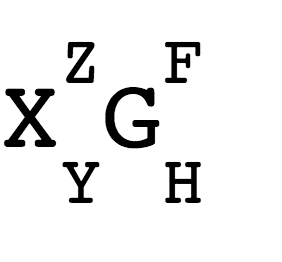
\includegraphics[width=0.3\columnwidth]{img/ej7.png}}{X\_Y\detokenize{^}ZG\detokenize{^}F\_H}
  \qquad
  \subsubfloat{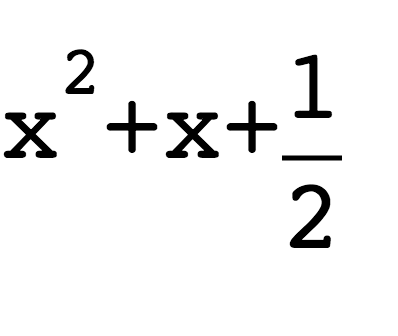
\includegraphics[width=0.3\columnwidth]{img/ej6.png}}{x\detokenize{^}2+x+\{1/2\}}
  \qquad
  \subsubfloat{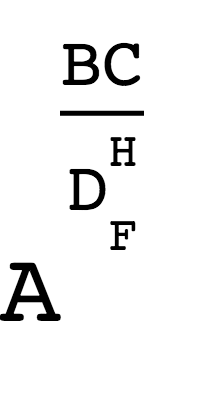
\includegraphics[width=0.3\columnwidth]{img/ej8.png}}{A\detokenize{^}\{BC/D\_F\detokenize{^}H\}}
  \end{minipage}}

\subfloat[]{
  \begin{minipage}{\columnwidth}\footnotesize
  \centering
  \subsubfloat{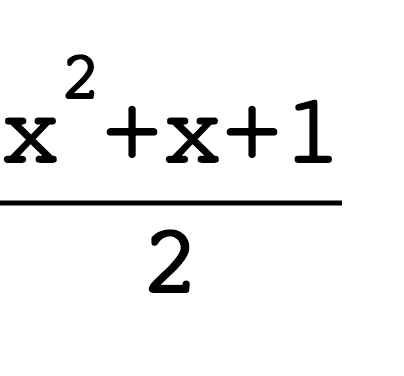
\includegraphics[width=0.3\columnwidth]{img/ej5.png}}{{x\detokenize{^}2+x+1}/2}
  \qquad
  \subsubfloat{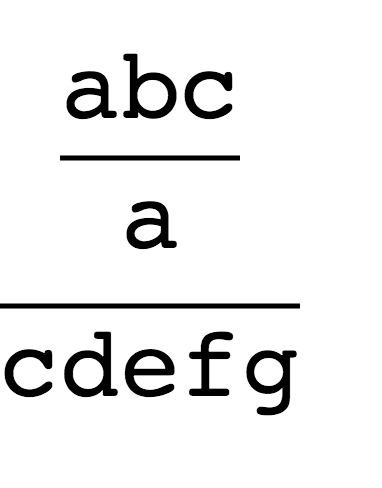
\includegraphics[width=0.3\columnwidth]{img/ej4.png}}{abc/a/cdefg}
  \qquad
  \subsubfloat{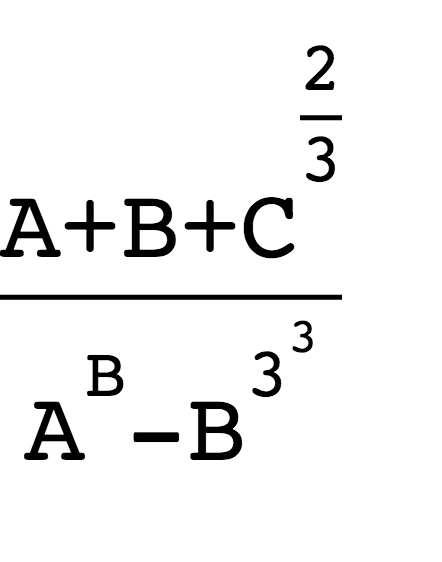
\includegraphics[width=0.3\columnwidth]{img/ej10.png}}{A+B+C\detokenize{^}\{2/3\}/\{A\detokenize{^}B-B\detokenize{^}\{3\detokenize{^}3\}\}}
  \end{minipage}
 }
\end{figure}

\begin{figure}[H]
\subfloat[]{
  \begin{minipage}{\columnwidth}\footnotesize
  \centering
  \subsubfloat{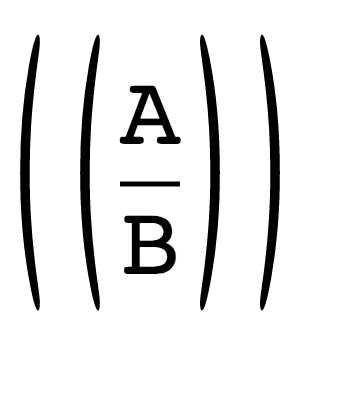
\includegraphics[width=0.3\columnwidth]{img/ej16.png}}{((A/B))}
  \qquad
  \subsubfloat{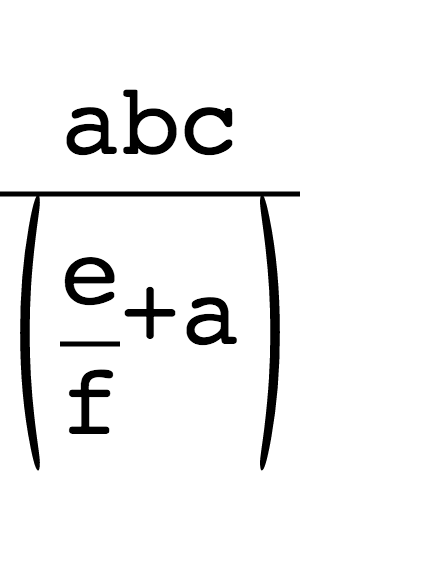
\includegraphics[width=0.3\columnwidth]{img/ej14.png}}{abc/(\{e/f\}+a)}
  \qquad
  \subsubfloat{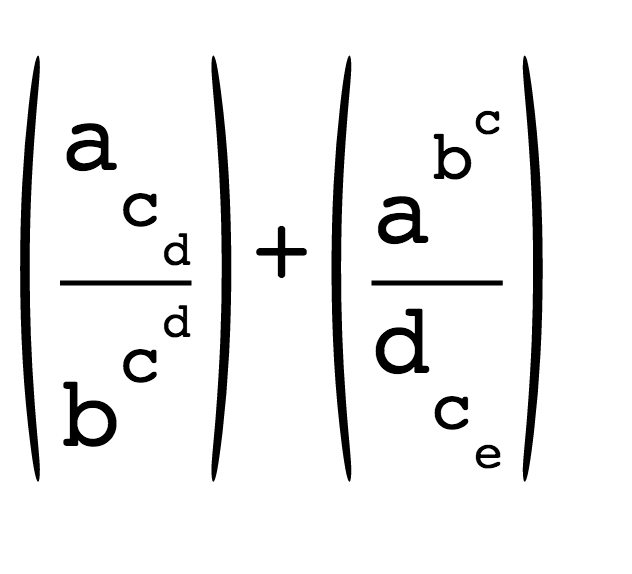
\includegraphics[width=0.3\columnwidth]{img/ej15.png}}{(\{a\_\{c\_d\}/b\detokenize{^}\{c\detokenize{^}d\}\})+(\{a\detokenize{^}\{b\detokenize{^}c\}/d\_\{c\_e\}\})}
  \end{minipage}
}

\subfloat[]{
  \begin{minipage}{\columnwidth}\footnotesize
  \centering
  \subsubfloat{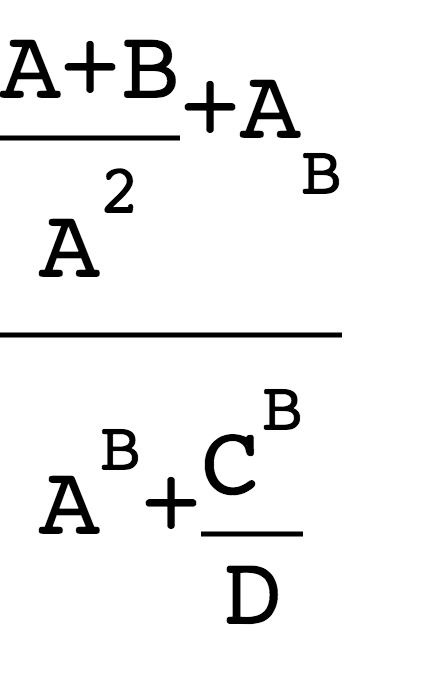
\includegraphics[width=0.3\columnwidth]{img/ej11.png}}{\{A+B/A\detokenize{^}2\}+A\_B/\{A\detokenize{^}B+\{C\detokenize{^}B/D\}}
  \qquad
  \subsubfloat{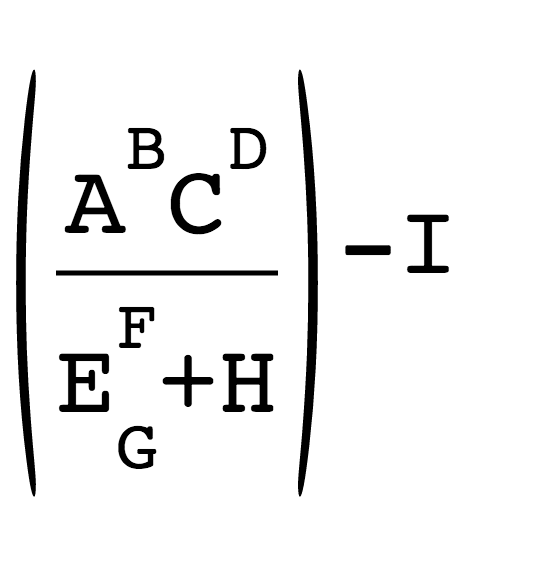
\includegraphics[width=0.3\columnwidth]{img/ej13.png}}{(A\detokenize{^}BC\detokenize{^}D/E\detokenize{^}F\_G+H)-I}
  \qquad
  \subsubfloat{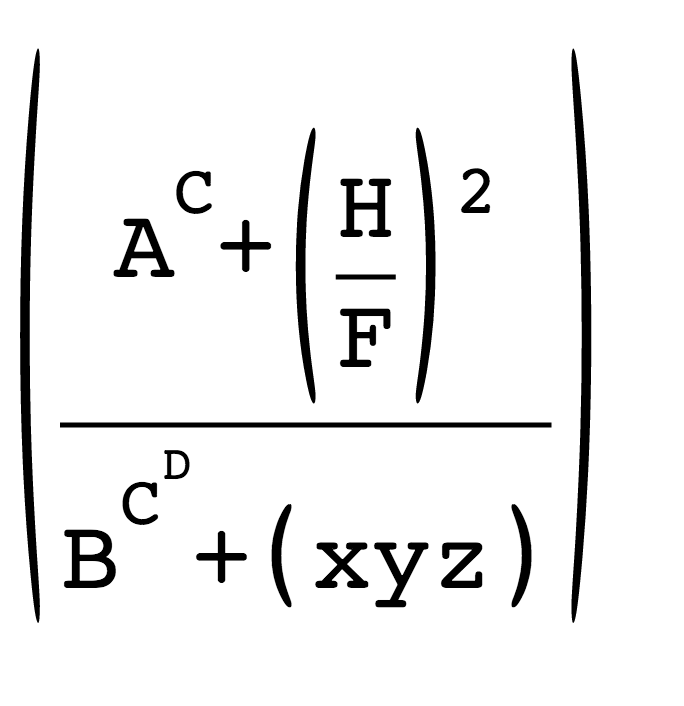
\includegraphics[width=0.3\columnwidth]{img/ej17.png}}{(A\detokenize{^}C+(H/F)\detokenize{^}2/B\detokenize{^}{C\detokenize{^}D}+(xyz))}
  \end{minipage}
 }
\end{figure}

A continuación exponemos algunos ejemplos de cadenas que no son aceptadas por el programa (debido a que no son aceptadas por la gramática usada):
\begin{table}[H]
  \begin{tabular}{|c|c|}
  \hline
  \{A & Error: Cadena no valida \\
  \hline
  A\detokenize{^}B\detokenize{^}C & Error: Cadena no valida \\
  \hline
  A\_B\_C & Error: Cadena no valida \\
  \hline
  A\_(B\_)C & Error: Cadena no valida \\
  \hline
  \end{tabular}
  \quad \quad \quad
  \begin{tabular}{|c|c|}
  \hline
  A//B & Error: Cadena no valida \\
  \hline
  () & Error: Cadena no valida \\
  \hline
  \{(\}) & Error: Cadena no valida \\
  \hline
  \{(AB\}AB) & Error: Cadena no valida \\
  \hline
  \end{tabular}

\end{table}


\section{Manual de usuario}
Para correr el TP, es necesario tener instalado Python 2.7 o posterior y la librería PLY, que puede obtenerse en https://pypi.python.org/pypi/ply. Para correr el tp, abrir una terminal en la carpeta src, y ejecutar el comando `` python tp.py ''. A continuación, introducir la cadena que se desea generar. Se genera la figura deseada con la extensión `` .svg '' en el archivo `` figura.svg ''.

\section{Conclusiones}
La realización de este Trabajo Práctico fue interesante, ya que nos permitió generar una aplicación concreta de toda la teoría vista en la segunda parte de la materia, básicamente sobre gramáticas de atributos y traducción dirigida por sintaxis (TDS). Entendimos mejor la relación que hay entre un árbol sintáctico, una gramática y una TDS para la generación de una herramienta de parsing de utilidad en la vida real.

Como se puede ver en los casos de test, las figuras que genera nuestro programa son de un nivel de calidad aceptable ya que en todos los casos expuestos se nota muy bien cuál es la expresión lógica-matemática que se pretende generar. Obviamente la herramienta podría ser mejorada para que las figuras queden `` más lindas '', pero por lo que vimos en el desarrollo del TP, esta no es una tarea fácil ya que para hacer esto hay que hacer mucha experimentación y fijar una gran variedad de parámetros y constantes para considerar la gran variedad de combinaciones que se pueden generar a partir los símbolos y la gramática considerada.


\section{Codigo}
\definecolor{keywords}{RGB}{255,0,90}
\definecolor{comments}{RGB}{0,0,113}
\definecolor{red}{RGB}{160,0,0}
\definecolor{green}{RGB}{0,150,0}

\lstset{language=Python,
        breaklines=true,
        basicstyle=\ttfamily\small,
        keywordstyle=\color{keywords},
        commentstyle=\color{comments},
        stringstyle=\color{red},
        showstringspaces=false,
        identifierstyle=\color{green},
        procnamekeys={def,class}}

\subsection{tp.py}
\lstinputlisting{../src/tp.py}

\subsection{parser_rules.py}
% \lstinputlisting{../src/parser_rules.py}
\begin{lstlisting}
from lexer_rules import tokens

from expressions import *

import pprint

def p_expression_init(subexpressions):
  'S : E'
  subexpressions[0] = Root(subexpressions[1])

# E -> E / A | A
def p_expression_E1(subexpressions):
  'E : E DIVIDE A'
  subexpressions[0] = Divide(subexpressions[1], subexpressions[3])

def p_expression_E2(subexpressions):
  'E : A'
  subexpressions[0] = subexpressions[1]

# A -> A B | B
def p_expression_A1(subexpressions):
  'A : A B'
  subexpressions[0] = Concat(subexpressions[1], subexpressions[2])

def p_expression_A2(subexpressions):
  'A : B'
  subexpressions[0] = subexpressions[1]

# B -> C | C SUPERINDEX C | C SUBINDEX C | C SUPERINDEX C SUBINDEX C | C SUBINDEX C SUPERINDEX C
def p_expression_B1(subexpressions):
  'B : C'
  subexpressions[0] = subexpressions[1]

def p_expressionB2(subexpressions):
  'B : C SUPERINDEX C'
  subexpressions[0] = SuperIndex(subexpressions[1], subexpressions[3])

def p_expressionB3(subexpressions):
  'B : C SUBINDEX C'
  subexpressions[0] = SubIndex(subexpressions[1], subexpressions[3])

def p_expressionB4(subexpressions):
  'B : C SUPERINDEX C SUBINDEX C'
  subexpressions[0] = SuperSubIndex(subexpressions[1], subexpressions[3], subexpressions[5])

def p_expressionB5(subexpressions):
  'B : C SUBINDEX C SUPERINDEX C'
  subexpressions[0] = SubSuperIndex(subexpressions[1], subexpressions[3], subexpressions[5])

# C -> { E }
def p_expression_C1(subexpressions):
  'C : LBRACKET E RBRACKET'
  subexpressions[0] = subexpressions[2]

# C -> ( E )
def p_expression_C2(subexpressions):
  'C : LPAREN E RPAREN'
  subexpressions[0] = Parenthesis(subexpressions[2])

# C -> ID
# tengo que escribir el valor del token ID
def p_expression_C3(subexpressions):
  'C : ID'
  subexpressions[0] = Id(subexpressions[1])

# Error rule for syntax errors
def p_error(p):
  raise Exception("Syntax error.")

\end{lstlisting}

\subsection{lexer_rules.py}
% \lstinputlisting{../src/lexer_rules.py}
\begin{lstlisting}
# Lista de tokens
tokens = [
    'ID',          # es hoja
    'DIVIDE',      # es nodo: /
    'LPAREN',      # es nodo: (
    'RPAREN',      # es nodo: )
    'LBRACKET',    # para separar expresiones sin agregar ningun simbolo
    'RBRACKET',    # para separar expresiones sin agregar ningun simbolo
    'SUPERINDEX',  # es nodo: ^
    'SUBINDEX'    # es nodo: _
]

# Expresiones regulares para cada token
t_ignore  = ' \t' # ignoramos los espacios
t_DIVIDE  = r'/'
t_LPAREN  = r'\('
t_RPAREN  = r'\)'
t_LBRACKET = r'\{'
t_RBRACKET = r'\}'
t_SUPERINDEX = r'\^'
t_SUBINDEX = r'\_'

def t_ID(t):
    r'[a-zA-Z0-9+-]'
    t.value = t.value
    return t


def t_error(t):
    message = "Token desconocido:"
    message += "\ntype:" + t.type
    message += "\nvalue:" + str(t.value)
    message += "\nline:" + str(t.lineno)
    message += "\nposition:" + str(t.lexpos)
    raise Exception(message)

\end{lstlisting}


\subsection{expressions.py}
\lstinputlisting{../src/expressions.py}




\end{document}
